\section{Security} Needles to say that the development process comes together with analyzing security vulnerabilities and implementing the solution to reduce them. My implementation contains two points where the setup plays a big role: the solution for storing sensitive data such as access and refresh tokens and the configuration of communication between the client and server sides.


\subsection{Tokens storage} Access and refresh tokens are both very sensitive pieces of data. In the case of successfully stealing the refresh token, an attacker will get long-term access to the application, or a short term in the case with the access token. That is why it is important to store these tokens as securely as it is possible.\\

\noindent \textbf{Most common attacks:} 

\begin{itemize}
    \item \emph{Cross-site scripting (XSS) attacks.} This is a type of attack where an attacker injects malicious scripts into a web page viewed by other users. It basically happens when an application trusts a user and the content, which can be inserted by them. 
    \item \emph{Cross-site request forgery (CSRF) attacks.} In general, this attack can be described as tricking a user into unintentionally performing some action. In this way, attackers just use the user's account to perform some harmful requests.
\end{itemize}


\noindent \textbf{Types of browser storages:} 

\begin{itemize}
    \item \emph{Local storage.} Local storage is web storage that allows the saving of key-value pairs of data. It provides the stored data persistence across the page reloading and can fit up to 5MB of data. Content from the local storage cannot be automatically sent and it makes it prone to CSRF attacks. However, it is not considered secure storage for keeping sensitive data due to the vulnerability to XSS attacks.
    \item \emph{Session storage} Session storage is client-base storage available by the browser which is very similar to the local storage. It has the same memory limit and vulnerabilities. But in addition to that it does not provide the persistence of data, which is a disadvantage to the user experience due to the need for repeated authentication.
    \item \emph{Cookies} Cookies are another way of storing data using a browser. Cookies can store much less data - up to 4KB, which might not always be enough for storing big tokens, but it is absolutely enough for my implementation. Cookies are vulnerable to both CSRF and XSS attacks, but with a proper configuration of secure attributes they are less vulnerable than local or session storage. Cookies can also be configured to be automatically sent with every HTTP request or some certain request.
\end{itemize}

\paragraph*{Solution for the refresh token.} The perfect solution for storing sensitive data in a browser does not exist and in order to keep the data secure there should be also implemented other vulnerability-reducing features like input data validation, escaping and others. However, with the proper use of security attributes, cookies are much more likely to mitigate those attacks. Moreover, using cookies for storing tokens is recommended by the OWASP community due to their secure configuration options. \\
I have come to the solution of storing the refresh token, which is the most sensitive token requiring persistence across page reloads, in httpOnly cookies. HttpOnly cookies must be set on the server side as they are not accessible for JavaSccirpt. Therefore, I had to adjust the implementation of sending and receiving the refresh token in the authentication microservice from the body of requests to cookies. Figure 4.5 shows the configuration of security attributes for the refresh token cookie.\\

\begin{figure}[h]
\centering
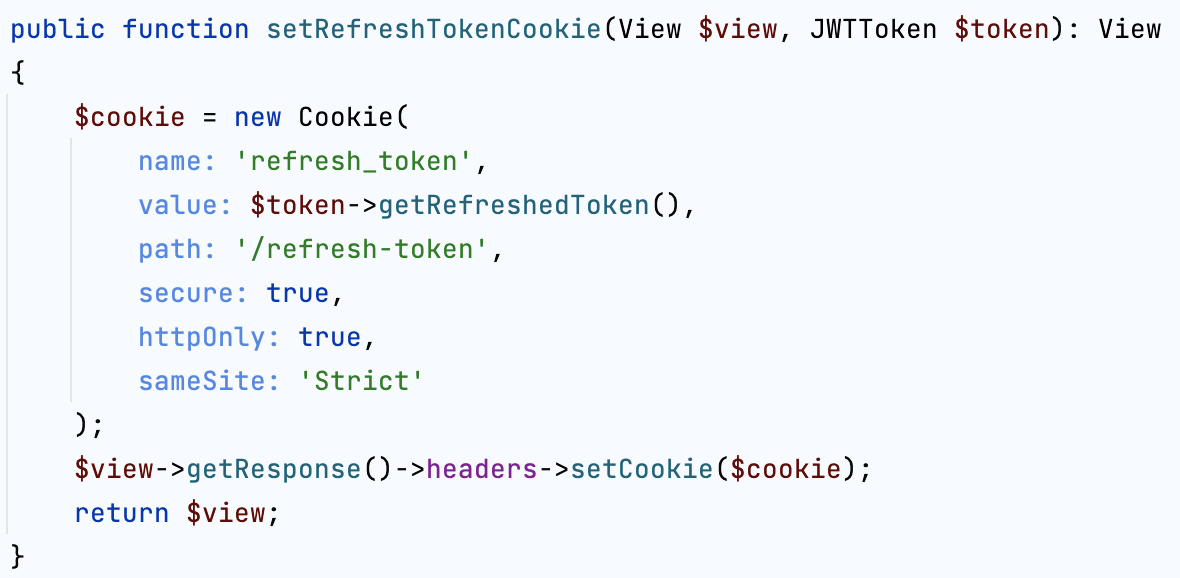
\includegraphics[scale=0.6]{../png/cookies.png}
\caption{Cookies setting}
\end{figure}

\noindent \textbf{Security attributes:}

\begin{itemize}
    \item \emph{Path.} URL path to which the cookie will be automatically sent.
    \item \emph{Secure.} This flag specifies that the cookie can be sent only through HTTPS ecrypted connections.
    \item \emph{HttpOnly.} The httpOnly flag is created to mitigate XSS attacks. With this flag, cookies can not be accessed by the Javascript.
    \item \emph{SameSite.} The strict value of that parameter means that the cookie is only sent if you are on the site that the cookie is set for. SameSite attribute is introduced for protection against CSRF. 
\end{itemize}


% https://www.invicti.com/learn/cookie-security-flags/

\paragraph*{Solution for the access token.} 

\subsection{Communication with the backend and CORS}
Cross-Origin Resource Sharing(CORS) is a security mef


